%%%%%%%%%%%%%%%%%%%%%%%%%%%%%%%%%%%%%%%%%
% Beamer Presentation
% LaTeX Template
% Version 1.0 (10/11/12)
%
% This template has been downloaded from:
% http://www.LaTeXTemplates.com
%
% License:
% CC BY-NC-SA 3.0 \ttp://creativecommons.org/licenses/by-nc-sa/3.0/)
%
%%%%%%%%%%%%%%%%%%%%%%%%%%%%%%%%%%%%%%%%%

%----------------------------------------------------------------------------------------
%	PACKAGES AND THEMES
%----------------------------------------------------------------------------------------

\documentclass[12pt]{beamer}
\usepackage[absolute,overlay]{textpos}

% small logo down the page
%\logo{\makebox[1\paperwidth]{
\includegraphics[width=.5cm,keepaspectratio]{images/sapienza-logo.png}}}

%\fontsize{12pt}{10}\selectfont



\usepackage{tikz}
%\setbeamertemplate{background canvas}{

%\begin{tikzpicture}
%\node[opacity=.1]{
%\includegraphics[width=2in , height=3in, keepaspectratio]%{images/sapienza-logo.png}};
%\end{tikzpicture}
%}
 % only for the image: http://ctan.org/pkg/mwe
%     \setbeamertemplate{background}{
\includegraphics[width=\paperwidth]{images/sapienza-logo.png}}
%{\usebackgroundtemplate{
%       \begin{picture}
%            
\includegraphics[width=\paperwidth]{images/sapienza-logo.png}
%       \end{picture}
%}%


% watermark logo , you can choose width and position in a pretty accurate way
%"anchor" and current page."x" play the game : north , south , etc.
\setbeamertemplate{background}{\tikz[overlay,remember picture, anchor=center]\node[opacity=.15]at ([yshift=0cm]current page.center){
\includegraphics[width=3cm]{images/sapienza-logo.png}};}


\definecolor{color1}{HTML}{001000} % Color of the article title and sections
\definecolor{color2}{HTML}{FF7a01} % Color of the boxes behind the abstract and headings
\definecolor{color3}{HTML}{202020} % Background color

\definecolor{baseColor}{HTML}{FF7a01} % Color of the boxes behind the abstract and headings
\mode<presentation> {

% The Beamer class comes with a number of default slide themes
% which change the colors and layouts of slides. Below this is a list
% of all the themes, uncomment each in turn to see what they look like.


%   \usetheme{Frankfurt}
%  \usetheme{Ilmenau}
%  \usetheme{JuanLesPins}
%  \usetheme{Luebeck}
%   \usetheme{PaloAlto}

\usetheme{Rochester}


% As well as themes, the Beamer class has a number of color themes
% for any slide theme. Uncomment each of these in turn to see how it
% changes the colors of your current slide theme.


% \usecolortheme{crane}
%\usecolortheme{orchid}
%   \usecolortheme{rose}
%  \usecolortheme{whale}


%\setbeamertemplate{footline} % To remove the footer line in all slides uncomment this line
\setbeamertemplate{footline}[page number] % To replace the footer line in all slides with a simple slide count uncomment this line

\setbeamertemplate{navigation symbols}{} % To remove the navigation symbols from the bottom of all slides uncomment this line

 \setbeamercolor*{palette primary}{use=structure,fg=color2,bg=color2!110 }
 \setbeamercolor*{palette secondary}{use=structure,fg=color3,bg=color3}
 \setbeamercolor{title}{fg=white,bg=baseColor!50!black}


}


\usepackage{graphicx} % Allows including images
\usepackage{booktabs} % Allows the use of \toprule, \midrule and \bottomrule in tables
\usepackage{scrextend}
\changefontsizes{11pt}
%----------------------------------------------------------------------------------------
%	TITLE PAGE
%----------------------------------------------------------------------------------------
\title[Short title]{Automated model-based android GUI testing using multi-level GUI Comparison Criteria} % The short title appears at the bottom of every slide, the full title is only on the title page

\author{happyBiker, haxxorrman} % Your name
\institute[Sapienza] % Your institution as it will appear on the bottom of every slide, may be shorthand to save space
{
Flatulenza, University of Prone \\ % Your institution for the title page
\medskip
\textit{homemadebike.9999999@stud.unipronax.fritt,} % Your email address
\textit{lexusGTsportage.99999999@stud.unipronax.fritt}

}
\date{\today} % Date, can be changed to a custom date

%%%%%%%%%%%%%%%%%%%%%%%%%%%%%%%%%%%%%%%%%%%%%%%%%
%%%   New style here

\mode<presentation>{\usetheme{AnnArbor}}
\usecolortheme{whale}

\setbeamercolor{frametitle}{parent=subsection in head/foot}
\setbeamercolor{frametitle right}{parent=section in head/foot}

\makeatletter
\pgfdeclarehorizontalshading[frametitle.bg,frametitle right.bg]{beamer@frametitleshade}{\paperheight}{%
    color(0pt)=(frametitle.bg);
    color(\paperwidth)=(frametitle right.bg)}

\AtBeginDocument{
    \pgfdeclareverticalshading{beamer@topshade}{\paperwidth}{%
        color(0pt)=(bg);
        color(4pt)=(black!50!bg)}
}

\addtobeamertemplate{headline}
{}
{%
    \vskip-0.2pt
    \pgfuseshading{beamer@topshade}
    \vskip-2pt
}


\setbeamertemplate{frametitle}
{%
    \nointerlineskip%
    \vskip-2pt%
    \hbox{\leavevmode
        \advance\beamer@leftmargin by -12bp%
        \advance\beamer@rightmargin by -12bp%
        \beamer@tempdim=\textwidth%
        \advance\beamer@tempdim by \beamer@leftmargin%
        \advance\beamer@tempdim by \beamer@rightmargin%
        \hskip-\Gm@lmargin\hbox{%
            \setbox\beamer@tempbox=\hbox{\begin{minipage}[b]{\paperwidth}%
                    \vbox{}\vskip-.75ex%
                    \leftskip0.3cm%
                    \rightskip0.3cm plus1fil\leavevmode
                    \insertframetitle%
                    \ifx\insertframesubtitle\@empty%
                    \strut\par%
                    \else
                    \par{\usebeamerfont*{framesubtitle}{\usebeamercolor[fg]{framesubtitle}\insertframesubtitle}\strut\par}%
                    \fi%
                    \nointerlineskip
                    \vbox{}%
                \end{minipage}}%
                \beamer@tempdim=\ht\beamer@tempbox%
                \advance\beamer@tempdim by 2pt%
                \begin{pgfpicture}{0pt}{0pt}{\paperwidth}{\beamer@tempdim}
                    \usebeamercolor{frametitle right}
                    \pgfpathrectangle{\pgfpointorigin}{\pgfpoint{\paperwidth}{\beamer@tempdim}}
                    \pgfusepath{clip}
                    \pgftext[left,base]{\pgfuseshading{beamer@frametitleshade}}
                \end{pgfpicture}
                \hskip-\paperwidth%
                \box\beamer@tempbox%
            }%
            \hskip-\Gm@rmargin%
        }%
        \nointerlineskip
        \vskip-0.2pt
        \hbox to\textwidth{\hskip-\Gm@lmargin\pgfuseshading{beamer@topshade}\hskip-\Gm@rmargin}
        \vskip-2pt
    }
\makeatother

\setbeamercolor{section in toc}{fg=red}
%%%

\setbeamercolor{structure}{fg=baseColor!80!black}
\setbeamercolor*{block title example}{fg=blue!50,bg= blue!10}
\setbeamercolor*{block body example}{fg= red,bg= blue!5}
\usefonttheme{structuresmallcapsserif}

\setbeamertemplate{footline}[page number]{} 

\setbeamercolor{headline}{fg=blue!90!black,bg=baseColor!90!black}
\setbeamercolor{palette primary}{fg=white,bg=baseColor!90!black}
\setbeamercolor{palette secondary}{fg=white,bg=baseColor!90!black}
\setbeamercolor{palette tertiary}{fg=white,bg=black}
\setbeamercolor{frametitle}{fg=white,bg=baseColor!50!black}


\colorlet{titleleft}{baseColor}
\colorlet{titleright}{black}

\setbeamercolor*{frametitle}{fg=white}

\makeatletter
\pgfdeclarehorizontalshading[titleleft,titleright]{beamer@frametitleshade}{\paperheight}{%
    color(0pt)=(titleleft);
    color(\paperwidth)=(titleright)}
\makeatother

%%%
%%%  End new style
%%%%%%%%%%%%%%%%%%%%%%%%%%%%%%%%%%%%%%%%%%%%%%%%




\begin{document}

\begin{frame}
\titlepage % Print the title page as the first slide
\end{frame}

\begin{frame}
\frametitle{Overview} % Table of contents slide, comment this block out to remove it
\tableofcontents % Throughout your presentation, if you choose to use \section{} and \subsection{} commands, these will automatically be printed on this slide as an overview of your presentation
\end{frame}

%----------------------------------------------------------------------------------------
%	PRESENTATION SLIDES
%----------------------------------------------------------------------------------------

%------------------------------------------------
%\section{Introduzione} % Sections can be created in order to organize your presentation into discrete blocks, all sections and subsections are automatically printed in the table of contents as an overview of the talk
%------------------------------------------------

%\begin{frame}
%    \frametitle{Introduzione}
%    In questa presentazione viene analizzato e riassunto il contentuto dell'articolo \textbf{``Automated Model-Based Android GUI Testing
%    using Multi-level GUI Comparison Criteria''} scritto da Young-Min Baek e Doo-Hwan Bae.
%\\~\\
%Presentazione preparata da 

%\end{frame}
\section{Introduzione}
\begin{frame}
    \frametitle{GUI testing automatico(1)}
    \begin{block}{Perch\`e dedicare particolare attenzione alle applicazioni Android?}
        Attualmente le applicazioni android comprendono quasi il 90\% del mercato di software mobile.

    \end{block}
    \begin{block}{Cos'\`e il GUI testing?}
        \`E una metodologia di testing che esplora una parte dello spazio degli stati del programma testato dando gli input al programma tramite l'interfaccia grafica.
    \end{block}
    \begin{block}{Perch\`e automatizzare il testing?}
        Il motivo principale \`e il costo, l'esecuzione manuale dei test ha il costo eccessivo per molte applicazioni.
        Inoltre l'esecuzione manuale dei test richiede tanto tempo e a volte non \`e in grado di individuare tutti gli errori.
    \end{block}


\end{frame}

\begin{frame}
    \frametitle{GUI testing automatico(2)}
Attualmente sul mercato si trovano dei tool per il GUI testing automatico che generano gli input in modo alleatorio, tentando di generare una sequenza di input che provoca il malfunzionamento del software.
Nel testo viene citato un tool chiamato \emph{Android Monkey} che permette questo tipo di test.
\\~\\
Dato che si tratta essenzialmente di una ricerca locale nello spazio degli stati, questi metodi sono soggetti alle problematiche degli algoritmi di ricerca locale. Per esempio possono valutare lo stesso stato pi\`u volte.
\\~\\
L'approccio proposto dagli autori \`e di costruire un grafo degli stati della GUI, utilizzando dei criteri di equivalenza (GUICC) per distinguere gli stati.
\end{frame}

\subsection{GUI Android}
\begin{frame}
    \frametitle{Modello GUI}
Un altro approccio prevede l'uso del modello della GUI.
Il modello GUI \`e un automa a stati finiti, dove gli stati dell'automa corrispondono agli stati dell'interfaccia grafica. L'automa transisce da uno stato all'altro al verificarsi di un evento.
Il modello GUI viene rappresentrato da un multigrafo dove i nodi corrispondono agli stati e gli archi corrispondono alle transizioni. Ogni arco \`e etichettato dall'evento che provoca la transizione.

Il concetto fondamentale necessario per la costruzione di questo grafo \`e il criterio di equivalenza degli stati.

\end{frame}

\begin{frame}{}

    Le applicazioni Android spesso generano parte dell'interfaccia grafica in modo dinamico.
    Per modellare correttamente la GUI biogna tener conto delle componenti dinamiche.

    \begin{figure}
    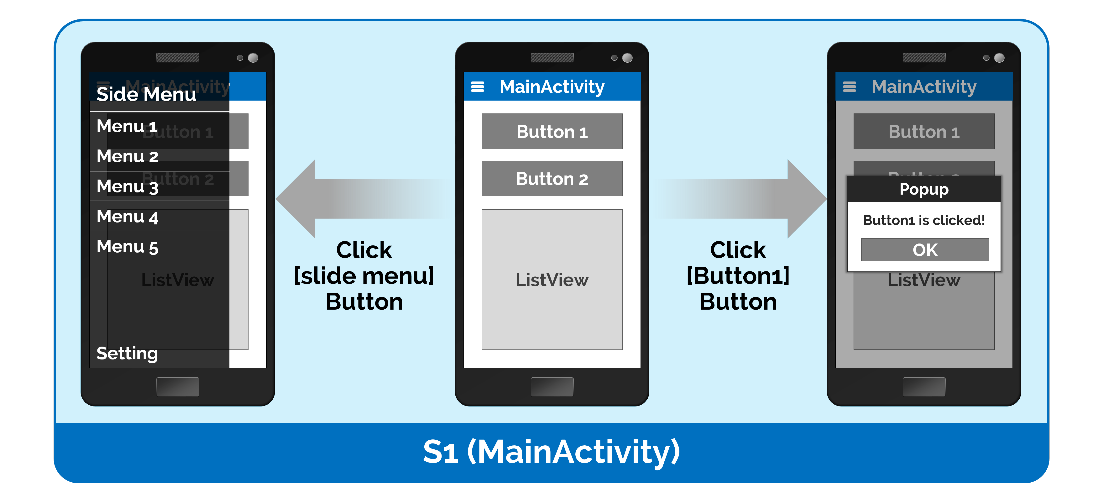
\includegraphics[width=0.8\linewidth]{images/Dynamic.png}
    \end{figure}
Un criterio d'equivalenza debole come "Nome Activity" in questo caso non sarebbe in grado di accorgersi della differenza tra gli stati.
\end{frame}

\begin{frame}
    \frametitle{Multi-Level
GUI Comparison Criteria (Multi-Level GUICC)}
La struttura a livelli definita dagli autori del paper \`e composta da:
\begin{itemize}
    \item \textbf{Nome pacchetto}. Quando l'activity corrente non appartiene allo stesso pacchetto dell'applicazione testata significa che l'applicazione testata \`e stata terminata oppure ha invocato un altra applicazione, in ogni caso lo stato corrente \`e considerato lo stato terminale.
    \item \textbf{Nome Activity}. Quando l'activity corrente ha un nome diverso da quella precedente si tratta di uno stato diverso.
    \item \textbf{Composizione Widget non-eseguibili}
    \item \textbf{Composizione Widget eseguibili}
    \item \textbf{Contenuti}
\end{itemize}
\end{frame}

\begin{frame}
    \frametitle{Generazione del modello}
Dato che le applicazioni Android in genere non contengono un modello della GUI costruito dallo sviluppatore \`e stato sviluppato un metodo per dedurre il modello (\emph{Model learning}) da un applicazione tramite \emph{reverse engineering}(\emph{GUI Ripping}).
\end{frame}

\begin{frame}
    \frametitle{Generazione del modello(2)}

Per costruire il grafo della GUI vengono eseguiti iterativamente questi passaggi:
\begin{itemize}
    \item Generare un evento amissibile nello stato corrente.
    \item Verificare tramite i criteri d'equivalenza se lo stato della GUI \`e cambiato.
        In caso affermativo ci sono tre casi:
        \begin{itemize}
            \item Il nuovo stato \`e gi\`a presente come nodo nel grafo. Allora si aggiunge un arco dallo stato precedente al nuovo stato etichettato dall'evento che porta in questo stato.
            \item Non esiste un nodo corrispondente, allora abbiamo scoperto uno stato nuovo. Viene generato un nuovo nodo e generato l'arco come nel primo caso.
            \item Lo stato risultato \`e uno stato terminale, allora l'applicazione \`e terminata in seguito all'evento.(Terminazione normale o anormale dovuta ad un errore/eccezione).
        \end{itemize}
        In caso contrario si aggiunge un \emph{loop}(un arco che origina e termina nello stesso nodo) etichettato dall'evento.

\end{itemize}

\end{frame}

\begin{frame}
    \frametitle{Architettura del sistema}
    \begin{block}{Motore di testing}
        Viene eseguito lato controllore.
        \begin{itemize}
            \item \textbf{Esecutore test} Sceglie l'input da mandare al software testato secondo un algoritmo(BFS).
            \item \textbf{Generatore del grafo} descritto sopra.
            \item \textbf{Error checker} Controlla la presenza di errori.
        \end{itemize}
    \end{block}
    \begin{block}{Strato di comunicazione}
        Serve per trasferire informazioni fra la macchina controllore e il dispositivo Android che esegue il software testato.
    \end{block}
    \begin{block}{Event agent}
        Software eseguito sul dispositivo Android. Riceve messaggi dal contollore e genera input al software testato corrispondenti.
    \end{block}
\end{frame}

%------------------------------------------------
%------------------------------------------------
%------------------------------------------------
%------------------------------------------------
%------------------------------------------------
%------------------------------------------------
%------------------------------------------------
%------------------------------------------------
%------------------------------------------------
%------------------------------------------------
%------------------------------------------------
%------------------------------------------------

%------------------------------------------------
{
\setbeamertemplate{background}{\tikz[overlay,remember picture, anchor=center]\node[opacity=1]at ([yshift=-0.5cm]current page.center){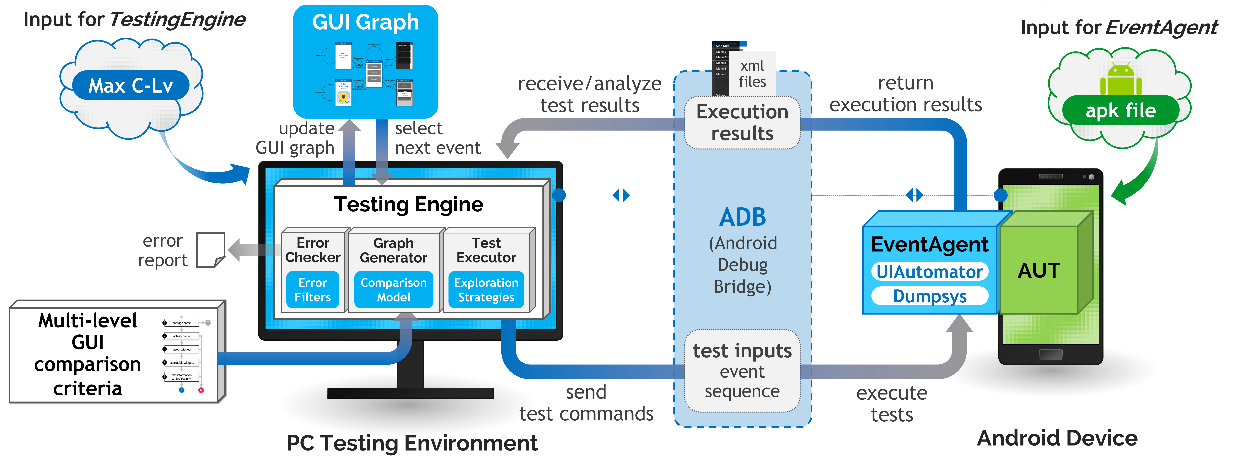
\includegraphics[width=0.9\linewidth]{images/framework.png}};}

\begin{frame}
    \frametitle{GUI Testing 1 : Funzionamento del framework}



\end{frame}
}
%------------------------------------------------
{
\setbeamertemplate{background}{\tikz[overlay,remember picture, anchor=center]\node[opacity=0.3]at ([yshift=-0.5cm]current page.center){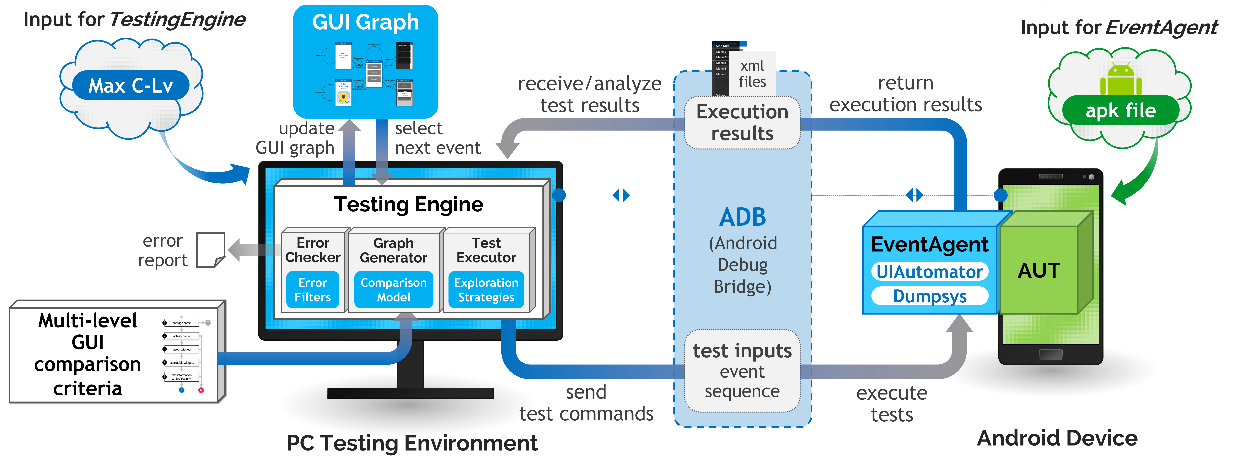
\includegraphics[width=0.9\linewidth]{images/framework.png}};}

\begin{frame}
\frametitle{GUI Testing 2 : input e output}
 figura in sfondo
    Questo framework riceve in input:
    \begin{itemize}
        \item file \textbf{Android APK} (eseguibile dell'App);
        \item \textbf{Max C-Lv},
    \end{itemize}
    \\~\\ 
    e restituisce in output:
    \begin{itemize}
        \item un insieme di \textbf{sequenze di eventi} , eseguite sull'applicazione ;
        \item un \textbf{grafo della GUI}, rappresentante gli stati esplorati e testati dell'app;
        \item un \textbf{error report}, se il framework ha riscontrato qualche errore nell'app ,
    \end{itemize}
    che \`e di fatto il fine ultimo del testing.


\end{frame}
}
%------------------------------------------------

\begin{frame}
\frametitle{Obiettivo: Scovare l'errore}
 
    Automatizzare il processo di error-detection nella GUI di una app porta vantaggi :
    \begin{enumerate}
        \item di tempo, perch\`e non bisogna testare manualmente ogni possibilit\`a;
        \item economici, perch\`e si evita che l' utente finale incappi in \textit{uncovered errors}, con ripercussioni sulla \textit{fame} dell'app.
    \end{enumerate}
    \\~\\
    Lo scopo del \textbf{model-based GUI testing} \`e di rilevare i \textit{runtime erros} in modo automaticizzato.
    \\~\\
    Ovviamente, migliore \`e il \textbf{modello} su cui si basa il GUI testing, maggiori sono le probabilit\`a di individuare tutti i possibili \textit{runtime errors}. 




\end{frame}

%------------------------------------------------

\begin{frame}
\frametitle{Sono utili i GUICC ?}

\begin{block}{Domanda 1}
In che modo i \emph{GUICC} influenzano la generazione di modelli di comportamento delle app Android ?
\end{block}

\begin{block}{Domanda 2}
    I GUICC influenzano la \textbf{copertura di codice} durante la fase di GUI testing  ? 
\end{block}

\begin{block}{Domanda 3}
I GUICC influenzano la capacit\`a di scovare errori durante la fase di GUI testing ?
\end{block}


\end{frame}

%------------------------------------------------

\begin{frame}
\frametitle{Domanda 1}

\begin{block}{Domanda 1}
In che modo i \emph{GUICC} influenzano la generazione di modelli di comportamento delle app Android ?
\end{block}

Sono state considerate varie apps, sia open source che proprietarie, e ne sono stati generati vari GUI graphs, ognuno basato su un diverso livello di "specificit\`a" dei GUICC .
\\~\\

Nella raccolta dei dati , i grafi generati con C-Lv 1 non sono stati considerati, poich\`e \`e un criterio troppo poco discriminante per ottenere risultati validi.
\\~\\

\begin{block}{Recall} 
\textit{\textbf{C-Lv 1}} : due ScreenNodes differiscono per il package di appartenenza.
\end{block}
\end{frame}

%------------------------------------------------

\begin{frame}
\frametitle{Grafi generati con vari Criteria Levels}

\begin{figure}
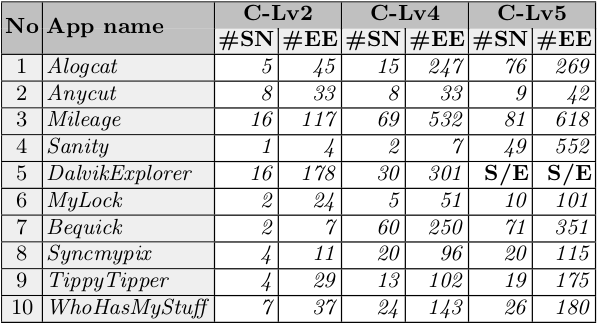
\includegraphics[width=0.55\linewidth]{images/GraphWidthForOpenSource.png}
\end{figure}
\begin{figure}
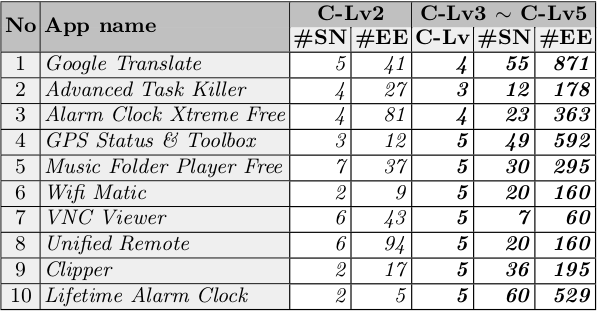
\includegraphics[width=0.55\linewidth]{images/GraphWidthForGstore.png}
\end{figure}
\end{frame}

%------------------------------------------------

\begin{frame}
\frametitle{Osservazioni}

\begin{itemize}
\item C-Lvs superiori generano pi\`u nodi e pi\`u archi ;

\item C-Lv 2 \`e un criterio meno "espressivo" di C-Lv5 ;

\item ATTENZIONE: app come X (per la gestione del ...) o come Davik (gestione dei processi) generano stati infiniti e il grafo esplode .

\end{itemize}

\end{frame}

%------------------------------------------------

\begin{frame}
\frametitle{Domanda 1}

\begin{block}{Domanda 1}
In che modo i \emph{GUICC} influenzano la generazione di modelli di comportamento delle app Android ?
\end{block} 
\begin{block}{Risposta}
Criteri pi\`u "specializzati" possono rendere il GUI states graph pi\`u completo ed esaustivo , ma livelli eccessivamente fine-grained di selezione non  migliorano la qualit\`a del grafo .
\end{block}

\end{frame}

%------------------------------------------------

\begin{frame}

\frametitle{Una semplice Calcolatrice ...}
\begin{figure}
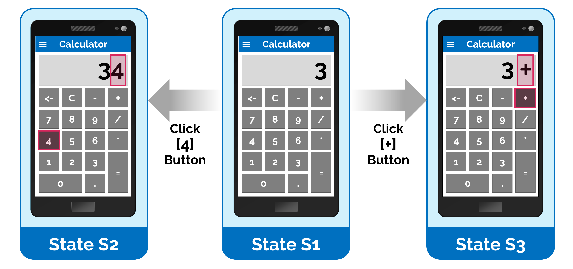
\includegraphics[width=0.8\linewidth]{images/calculator.png}
\end{figure}
Una calcolatrice \`e una app particolare : \`e indistinguibile per ogni \textbf{C-Lv} precedente al quinto
\\~\\
Quando si inizia a comparare \textbf{in base al testo inserito} per\`o il numero di stati esplode : ogni nuovo carattere (numero o operatore) inserito corrisponde ad un nuovo ScreenNode.
\end{frame} 

%------------------------------------------------

\begin{frame}
\frametitle{Wider is not better ...}
Testare applicazioni simili a Calculator \textbf{\textit{ \`e complicato}} , poich\`e pi\`u specifico \`e \textbf{Max C-Lv} , pi\`u grande \`e il grafo risultante.
\\~\\

Grafi molto grandi talvolta contengono ScreenNodes diversi da cui possono essere avviati eventi uguali , quindi i test perdono molto tempo su input simili.
\\~\\

Inoltre non \`e detto che con grafi pi\`u grandi si riescano a coprire tutte le funzionalit\`a messe a disposizione da un'app. 
\end{frame}

%------------------------------------------------

\begin{frame}
\frametitle{Come misurare oggettivamente la quantit\`a di funzionalit\`a testate ?}
Per avere una misura oggettiva del numero di funzionalit\`a testate , si pu\`o misurare il numero di linee di codice effettivamente eseguite durante un test sul grafo .
\\~\\

In generale , maggiore \`e il numero di linee di codice eseguite , maggiore \`e il numero di funzionalit\`a testate.
\end{frame}

%------------------------------------------------

\begin{frame}
\frametitle{Domanda 2}
\begin{block}{Domanda 2}
    I GUICC influenzano la \textbf{copertura di codice} durante la fase di GUI testing  ? 
\end{block}
\\~\\

I test sono stati effettuati sempre sullo stesso insieme di app open source e proprietarie.

\end{frame}

%------------------------------------------------

\begin{frame}
\frametitle{Linee di codice eseeguite nelle App testate}
\begin{figure}
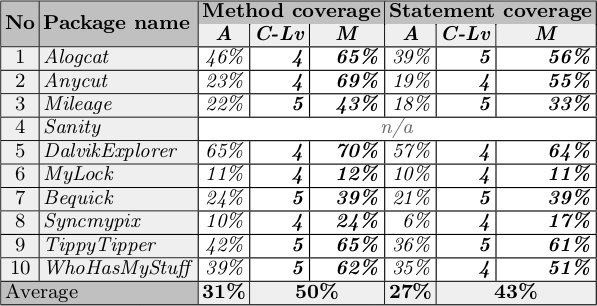
\includegraphics[width=0.8\linewidth]{images/LOCcoverage.png}
\end{figure}
\end{frame}

%------------------------------------------------

\begin{frame}
\frametitle{Osservazioni}
%(grafico risultati sullo sfondo)

\begin{itemize}
\item le colonne "A" contengono la percentuale di codice eseguito durante un test con Max C-Lv pari a 2 , ossia test eseguiti con il criterio degli activity name;

\item le colonne "C-Lv" e "M" vanno lette insieme : "C-Lv" indica il livello a cui viene raggiunta la massima percentuale di codice eseguito "M";

\item ci sono alcune eccezioni , dovute per\`o a specifici casi particolari;

\item si nota chiaramente che livelli pi\`u specializzati di GUICC coprono una maggior percentuale di codice eseguito
\end{itemize}


\end{frame}

%------------------------------------------------

\begin{frame}
\frametitle{Domanda 2}
\begin{block}{Domanda 2}
    I GUICC influenzano la \textbf{copertura di codice} durante la fase di GUI testing  ? 
\end{block}

\begin{block}{Risposta}
Il livello di GUICC influenza in modo significativo la percentuale di codice eseguito .
\end{block}

\end{frame}

%------------------------------------------------


\begin{frame}
\frametitle{Domanda 3}

\begin{block}{Domanda 3}
I GUICC influenzano la capacit\`a di scovare errori durante la fase di GUI testing ?
\end{block}


\end{frame}

%------------------------------------------------
\begin{frame}
\frametitle{Runtime errors}
\begin{figure}
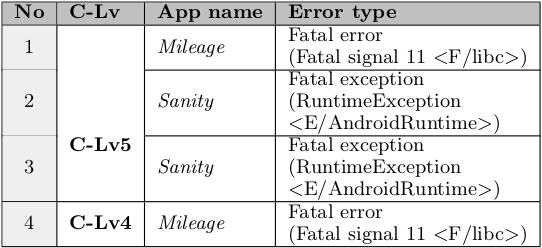
\includegraphics[width=0.8\linewidth]{images/errors.png}
\end{figure}

\begin{itemize}
\item 4 tipi di errori fondamentali ;
\item tutti rilevati con grafi "fine-grained" , ossia con criteri di comparazione a basso livello (C-Lv 4/5) .

\end{itemize}

\end{frame}

%------------------------------------------------
\begin{frame}
\frametitle{Domanda 3}

\begin{block}{Domanda 3}
I GUICC influenzano la capacit\`a di scovare errori durante la fase di GUI testing  ?
\end{block}

\begin{block}{Risposta}
Oltre a influenzare la quantit\`a di codice eseguito ,  il livello di GUICC influenza anche molto la capacit\`a di "error detection" del test.
\end{block}

\end{frame}

%------------------------------------------------
\begin{frame}
\frametitle{Conclusione}
La maggior parte delle tecniche di \textit{model-based Android GUI testing} esistenti non ha possibilit\`a di utilizzo pratico, poich\`e vengono trascurati alcuni comportamenti dinamici frequenti nelle applicazioni moderne.
\\~\\
Questo \`e il primo studio che si \`e concentrato sulla \textit{valutazione della generazione del modello} pi\`u che sulla applicazione del modello stesso su un qualche framework.
\\~\\
Da questa valutazione \`e emerso che i GUI Comparison Criteria sono molto vantaggiosi : si pu\`o scegliere il grado di dettaglio di un test (modificando il \textbf{Max C-Lv}) ed \`e possibile coprire un'alta percentuale di linee di codice eseguite , rilevando una altrettanto alta percentuale di \textbf{runtime errors}.
\\~\\
Manca un metodo che selezioni , per una data app , quali Comparison Criteria siano pi\`u adeguati per ottenere una pi\`u vasta copertura di codice e di errori. Tale metodo sar\`a oggetto di ricerca futura.


\end{frame}

%------------------------------------------------


\end{document} 
